\documentclass{article}
\usepackage{pgfplots}
\pgfplotsset{compat=newest}

\begin{document}

\begin{figure}[h]
    \centering
    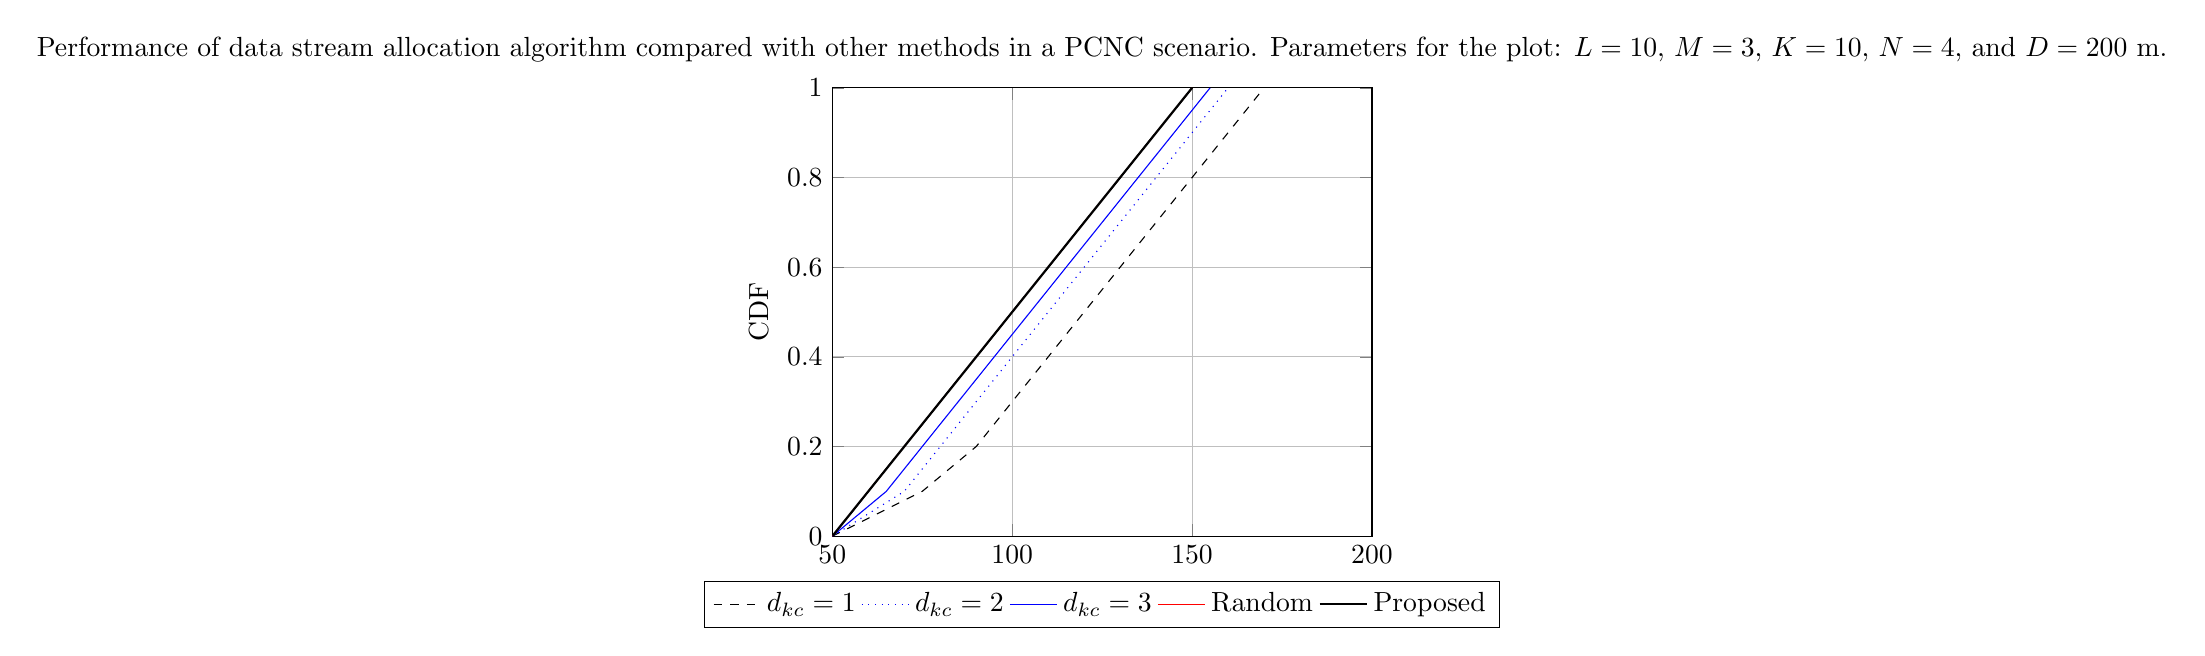
\begin{tikzpicture}
        \begin{axis}[
            xlabel={Sum Rate (bpcu)},
            ylabel={CDF},
            xmin=50,
            xmax=200,
            ymin=0,
            ymax=1,
            xtick={50, 100, 150, 200},
            ytick={0, 0.2, 0.4, 0.6, 0.8, 1},
            legend pos=south east,
            grid=major,
            title style={align=center},
            title={Performance of data stream allocation algorithm compared with other methods in a PCNC scenario. Parameters for the plot: $L=10$, $M=3$, $K=10$, $N=4$, and $D=200$~m.},
            legend entries={$d_{kc}=1$, $d_{kc}=2$, $d_{kc}=3$, Random, Proposed},
            legend cell align={left},
            legend style={at={(0.5,-0.1)}, anchor=north, legend columns=-1},
            ]
            \addplot [dashed, black] coordinates {
                (50,0) (75,0.1) (90,0.2) (100,0.3) (110,0.4) (120,0.5) (130,0.6) (140,0.7) (150,0.8) (160,0.9) (170,1)
            };
            \addplot [dotted, blue] coordinates {
                (50,0) (70,0.1) (80,0.2) (90,0.3) (100,0.4) (110,0.5) (120,0.6) (130,0.7) (140,0.8) (150,0.9) (160,1)
            };
            \addplot [solid, blue] coordinates {
                (50,0) (65,0.1) (75,0.2) (85,0.3) (95,0.4) (105,0.5) (115,0.6) (125,0.7) (135,0.8) (145,0.9) (155,1)
            };
            \addplot [solid, red] coordinates {
                (50,0) (60,0.1) (70,0.2) (80,0.3) (90,0.4) (100,0.5) (110,0.6) (120,0.7) (130,0.8) (140,0.9) (150,1)
            };
            \addplot [solid, thick, black] coordinates {
                (50,0) (60,0.1) (70,0.2) (80,0.3) (90,0.4) (100,0.5) (110,0.6) (120,0.7) (130,0.8) (140,0.9) (150,1)
            };
        \end{axis}
    \end{tikzpicture}
    \caption{Performance of data stream allocation algorithm compared with other methods in a PCNC scenario. Parameters for the plot: $L=10$, $M=3$, $K=10$, $N=4$, and $D=200$~m.}
    \label{fig:performance_comparison}
\end{figure}

\end{document}